\begin{figure}[H]
  \centering
  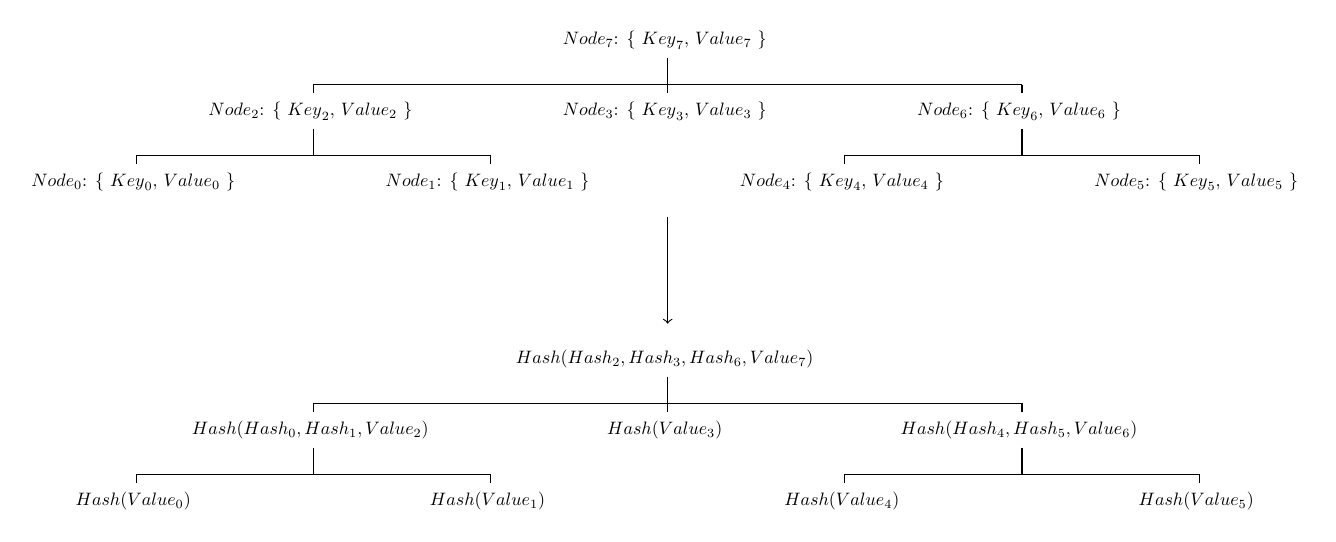
\begin{tikzpicture}[scale = 0.45, every node/.style={scale = 0.65}, every node/.append style={fill = white, rounded corners = 2pt, inner sep = 2pt, align = center}]

  \node at (0, 0) { $\text{Node}_7$: \{ $\text{Key}_7$, $\text{Value}_7$ \} };

  \draw (0, -0.5) -- (0, -1.5);
  \draw (-10, -1.25) -- (10, -1.25);
  \draw (-10, -1.25) -- (-10, -1.5);
  \draw (10, -1.25) -- (10, -1.5);

  \node at (-10, -2) { $\text{Node}_2$: \{ $\text{Key}_2$, $\text{Value}_2$ \} };
  \node at (0, -2) { $\text{Node}_3$: \{ $\text{Key}_3$, $\text{Value}_3$ \} };
  \node at (10, -2) { $\text{Node}_6$: \{ $\text{Key}_6$, $\text{Value}_6$ \} };

  \draw (-10, -2.5) -- (-10, -3.25);
  \draw (-15, -3.25) -- (-5, -3.25);
  \draw (-15, -3.25) -- (-15, -3.5);
  \draw (-5, -3.25) -- (-5, -3.5);

  \draw (10, -2.5) -- (10, -3.25);
  \draw (15, -3.25) -- (5, -3.25);
  \draw (15, -3.25) -- (15, -3.5);
  \draw (5, -3.25) -- (5, -3.5);

  \node at (-15, -4) { $\text{Node}_0$: \{ $\text{Key}_0$, $\text{Value}_0$ \} };
  \node at (-5, -4) { $\text{Node}_1$: \{ $\text{Key}_1$, $\text{Value}_1$ \} };

  \node at (5, -4) { $\text{Node}_4$: \{ $\text{Key}_4$, $\text{Value}_4$ \} };
  \node at (15, -4) { $\text{Node}_5$: \{ $\text{Key}_5$, $\text{Value}_5$ \} };

  \draw [ -> ] (0, -5) -- (0, -8);

  \node at (0, -9) { $\text{Hash}(\text{Hash}_2, \text{Hash}_3, \text{Hash}_6, \text{Value}_7)$ };

  \draw (0, -9.5) -- (0, -10.5);
  \draw (-10, -10.25) -- (10, -10.25);
  \draw (-10, -10.25) -- (-10, -10.5);
  \draw (10, -10.25) -- (10, -10.5);

  \node at (-10, -11) { $\text{Hash}(\text{Hash}_0, \text{Hash}_1, \text{Value}_2)$ };
  \node at (0, -11) { $\text{Hash}(\text{Value}_3)$ };
  \node at (10, -11) { $\text{Hash}(\text{Hash}_4, \text{Hash}_5, \text{Value}_6)$ };

  \draw (-10, -11.5) -- (-10, -12.25);
  \draw (-15, -12.25) -- (-5, -12.25);
  \draw (-15, -12.25) -- (-15, -12.5);
  \draw (-5, -12.25) -- (-5, -12.5);

  \draw (10, -11.5) -- (10, -12.25);
  \draw (15, -12.25) -- (5, -12.25);
  \draw (15, -12.25) -- (15, -12.5);
  \draw (5, -12.25) -- (5, -12.5);

  \node at (-15, -13) { $\text{Hash}(\text{Value}_0)$ };
  \node at (-5, -13) { $\text{Hash}(\text{Value}_1)$ };

  \node at (5, -13) { $\text{Hash}(\text{Value}_4)$ };
  \node at (15, -13) { $\text{Hash}(\text{Value}_5)$ };

  \end{tikzpicture}
  \caption{
    Example merkle tree
  }
  \label{fig:example_merkle_tree}
\end{figure}
